% Procedure for installation

\stepcounter{tableCounter} % Increment counter
\setcounter{rowCounter}{0} % Reset counter
\begin{tabularx}{\textwidth}{|>{\columncolor{tableColumnColor}}c|>{\columncolor{tableColumnColor}}c|>{\hsize=1.2\hsize}X|>{\hsize=.8\hsize}X|}
  \hline
  \rowcolor{tableHeaderColor}
  ID & Check & Description & Comments \\ \hline

  \procedureItem{Position the trailer such that the wheels are on the edge of the concrete ground. Also check the distance to the Hunter Stübli because of the cable length. Use safety map as orientation. 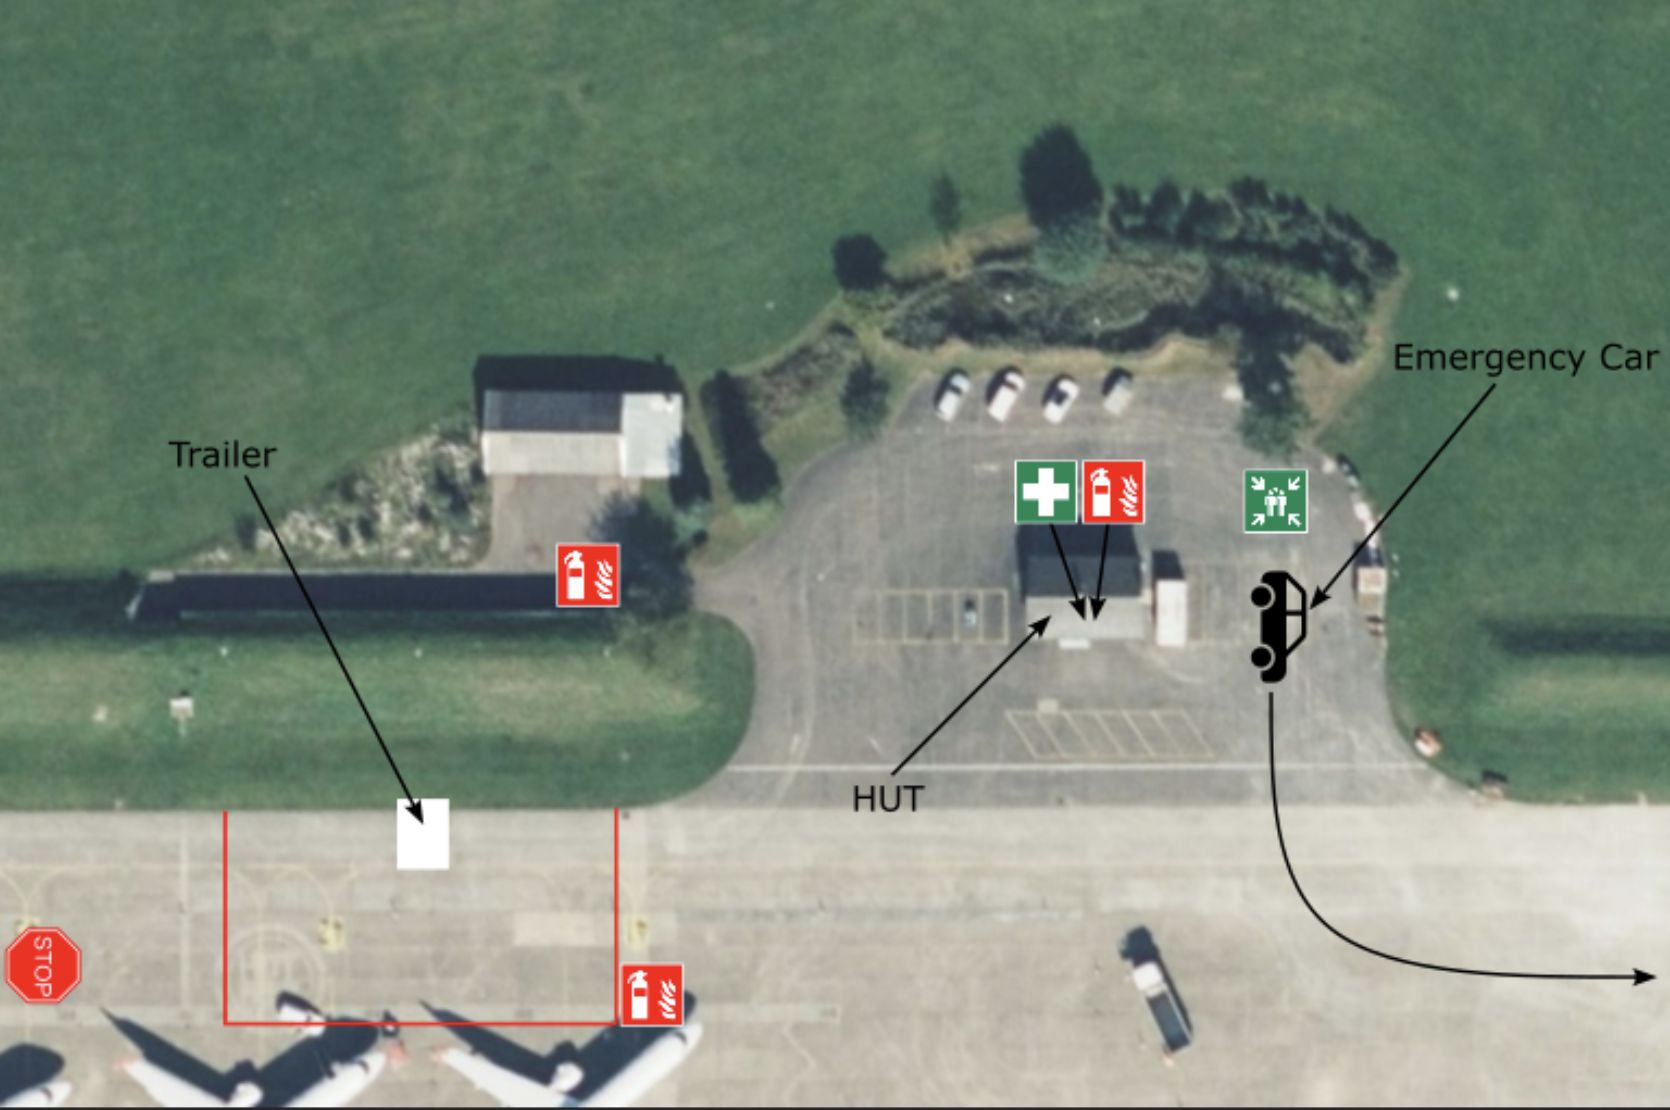
\includegraphics[width=\linewidth]{assets/position_map.png} }{}
  
  \procedureItem{Pull the brake of the trailer}{}
  
  \procedureItem{Put side covers up}{}
  
  \procedureItem{Place the “Riffelblech” on the grass under the front legs.}{}
  
  \procedureItem{Crank down the trailer legs until they carry the weight of the trailer}{}
  
  \procedureItem{Make sure that the shorter side of the Trailer is level (check with level at engine compartment)}{}
  
  \procedureItem{Make sure that the longer side of the Trailer is tilted slightly (mark on level) towards the engine compartment. (Check with level at both sides of the trailer)}{}
  
  \procedureItem{Install fixation cord on the frontside of the trailer by wrapping them once around the metal structures.}{}
  
  \procedureItem{Pull them slightly sidewards to the grass. If Spirafix is not installed: screw Spirafix into the ground where the cords end (hammer may be useful)}{}
  
  \procedureItem{Tighten fixation cord}{}
  
  \procedureItem{Check that trailer fixation is complete}{}
  
  \procedureItem{Inform TC \& PSS1}{}
  
\end{tabularx}
